\documentclass[DIV=calc, paper=a4, fontsize=11pt, twocolumn]{scrartcl}	 % A4 paper and 11pt font size

\usepackage{multirow}
\usepackage{graphicx}
\usepackage{lipsum} % Used for inserting dummy 'Lorem ipsum' text into the template
\usepackage[english]{babel} % English language/hyphenation
\usepackage[protrusion=true,expansion=true]{microtype} % Better typography
\usepackage{amsmath,amsfonts,amsthm} % Math packages
\usepackage[svgnames]{xcolor} % Enabling colors by their 'svgnames'
\usepackage[hang, small,labelfont=bf,up,textfont=it,up]{caption} % Custom captions under/above floats in tables or figures
\usepackage{booktabs} % Horizontal rules in tables
\usepackage{fix-cm}	 % Custom font sizes - used for the initial letter in the document

\usepackage{sectsty} % Enables custom section titles
\allsectionsfont{\usefont{OT1}{phv}{b}{n}} % Change the font of all section commands

\usepackage{fancyhdr} % Needed to define custom headers/footers
\pagestyle{fancy} % Enables the custom headers/footers
\usepackage{lastpage} % Used to determine the number of pages in the document (for "Page X of Total")

% Headers - all currently empty
\lhead{}
\chead{}
\rhead{}

% Footers
\lfoot{}
\cfoot{}
\rfoot{\footnotesize Page \thepage\ of \pageref{LastPage}} % "Page 1 of 2"

\renewcommand{\headrulewidth}{0.0pt} % No header rule
\renewcommand{\footrulewidth}{0.4pt} % Thin footer rule

\usepackage{lettrine} % Package to accentuate the first letter of the text
\newcommand{\initial}[1]{ % Defines the command and style for the first letter
\lettrine[lines=3,lhang=0.3,nindent=0em]{
\color{DarkGoldenrod}
{\textsf{#1}}}{}}

%----------------------------------------------------------------------------------------
%	TITLE SECTION
%----------------------------------------------------------------------------------------

\usepackage{titling} % Allows custom title configuration

\newcommand{\HorRule}{\color{DarkGoldenrod} \rule{\linewidth}{1pt}} % Defines the gold horizontal rule around the title

\pretitle{\vspace{-30pt} \begin{flushleft} \HorRule \fontsize{20}{20} \usefont{OT1}{phv}{b}{n} \color{DarkRed} \selectfont} % Horizontal rule before the title

\title{Sobel Filter for Edge Detection using VHDL} % Your article title

\posttitle{\par\end{flushleft}\vskip 0.5em} % Whitespace under the title

\preauthor{\begin{flushleft}\large \lineskip 0.5em \usefont{OT1}{phv}{b}{sl} \color{DarkRed}} % Author font configuration

\author{Ali Alipour, } % Your name

\postauthor{\footnotesize \usefont{OT1}{phv}{m}{sl} \color{Black} % Configuration for the institution name
University of Tehran % Your institution

\par\end{flushleft}\HorRule} % Horizontal rule after the title

\date{} % Add a date here if you would like one to appear underneath the title block

%----------------------------------------------------------------------------------------

\begin{document}

\maketitle % Print the title

\thispagestyle{fancy} % Enabling the custom headers/footers for the first page 

%----------------------------------------------------------------------------------------
%	ABSTRACT
%----------------------------------------------------------------------------------------

% The first character should be within \initial{}
\initial{T}\textbf{his project implements the Sobel Filter, an edge detection algorithm, 
using VHDL to process images efficiently. Edge detection is a crucial step in image processing, 
often used to highlight significant changes in intensity, which correspond to object boundaries within
 an image. The Sobel Filter is well-known for its ability to detect vertical and horizontal edges.}

%----------------------------------------------------------------------------------------
%	ARTICLE CONTENTS
%----------------------------------------------------------------------------------------

\section*{\small{Filter Design}}

% \lipsum[1-3] % Dummy text

The Sobel Filter was designed to detect both horizontal and vertical edges by applying two 3x3 kernels 
to the input image. One kernel detects horizontal changes in intensity, while the other detects vertical 
changes. The convolution process outputs a new image highlighting areas with significant intensity shifts. 
(See Figure 1 for the process of edge detection).

\begin{figure}[htbp]
  \centering
  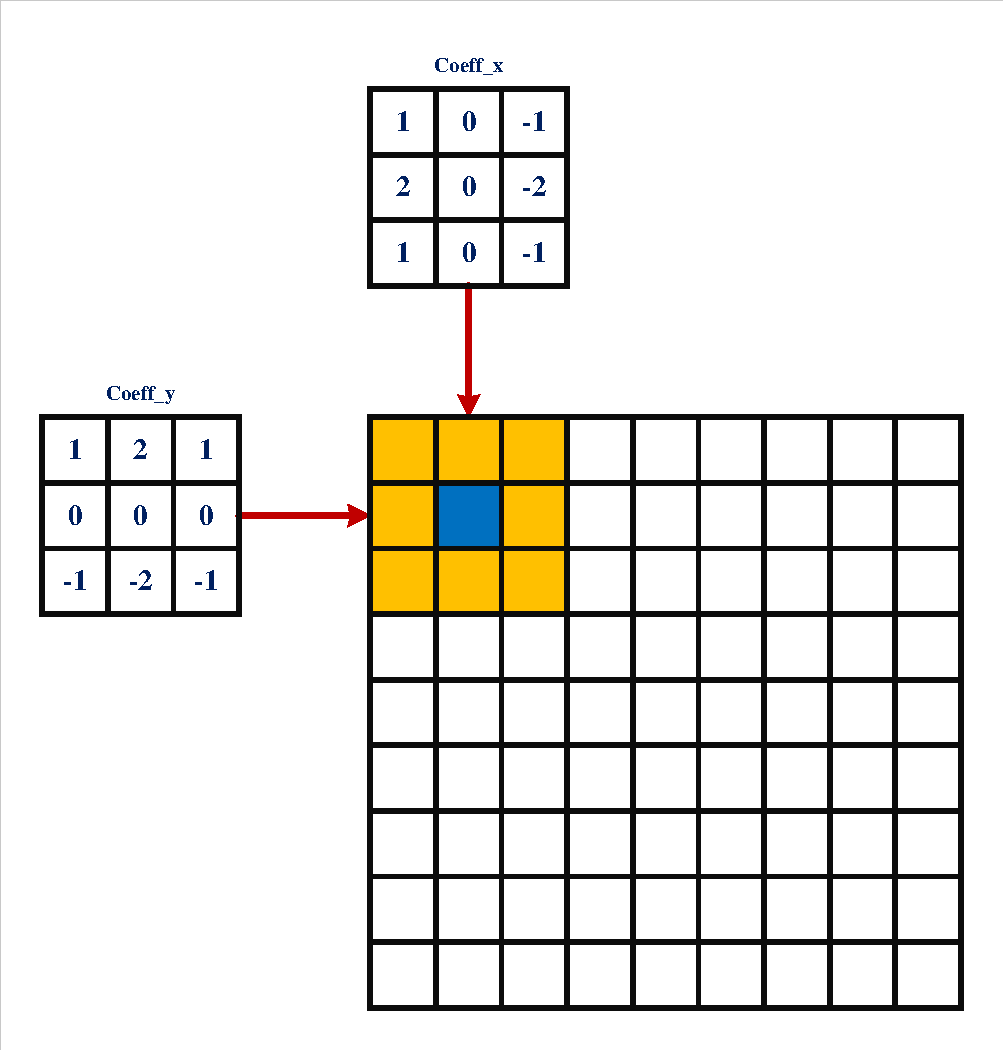
\includegraphics[width=0.4\textwidth]{C:\\Users\\USER\\Documents\\edit_project\\Sobel_Filter\\visio1.pdf}
  \caption{Figure 1}
  \label{fig:visio-diagram}
\end{figure}

% \begin{align}
% A = 
% \begin{bmatrix}
% A_{11} & A_{21} \\
% A_{21} & A_{22}
% \end{bmatrix}
% \end{align}

% \lipsum[4] % Dummy text

%------------------------------------------------
\section*{\small{Hardware Integration}}

% \lipsum[1-3] % Dummy text

\small{The hardware design includes the following components:}
\begin{itemize}
  \item \textbf{VHDL Modules:} The core modules of the filter, including the convolution operator and gradient calculations, 
                               were implemented in VHDL. These modules are responsible for calculating the Sobel Filter's output 
                               by processing each pixel in the input image.
  
  \item \textbf{Memory Management:} The memory read and write modules ensure that the input image is fetched from memory, processed 
                                    by the filter, and then the output image is written back to memory. This data flow is crucial for 
                                    real-time image processing.
\end{itemize}

% \[
% x = x^l \times 2^{l} + x^h
% \]

% Encoding types
% \textcolor{DarkRed}{Type 1 Encoding } \hspace{2cm} \textcolor{DarkGreen}{Type 2 Encoding }

\section*{\small{Methodology}}

% \lipsum[8] % Dummy text

Input pixels are sequentially read from memory, and once 9 pixels are retrieved, the matrix mapping operation is executed. 
The calculated result is then output, followed by the write command to store it back into memory. Figure 1 illustrates how 
the module receives the input, while Figure 2 displays the state machine designed for this filter.

\begin{figure}[htbp]
  \centering
  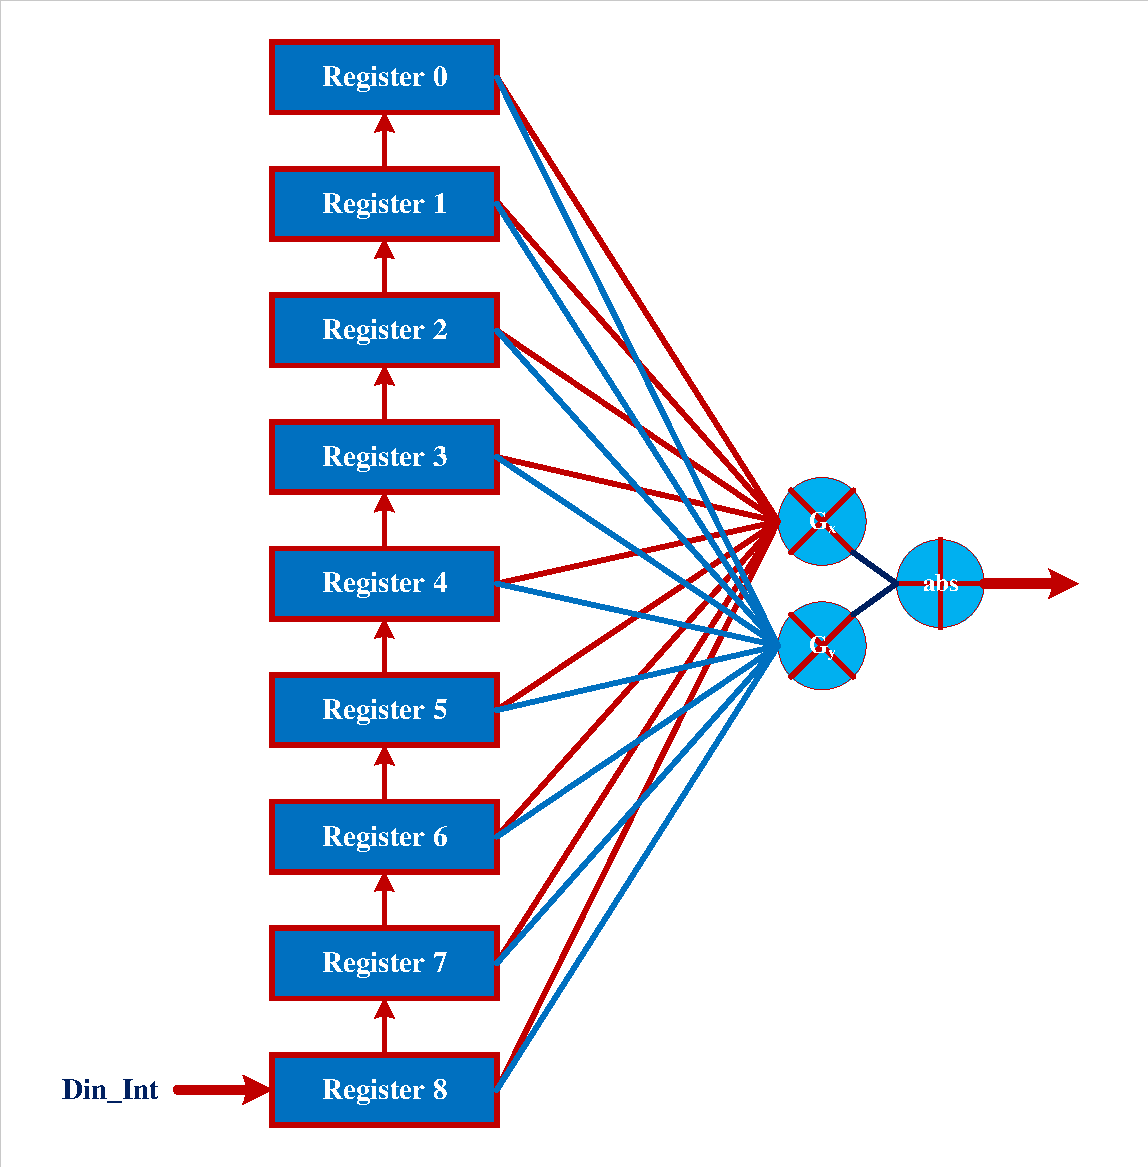
\includegraphics[width=0.4\textwidth]{C:\\Users\\USER\\Documents\\edit_project\\Sobel_Filter\\visio2.pdf}
  \caption{Figure 2}
  \label{fig:visio-diagram}
\end{figure}

\begin{figure}[htbp]
  \centering
  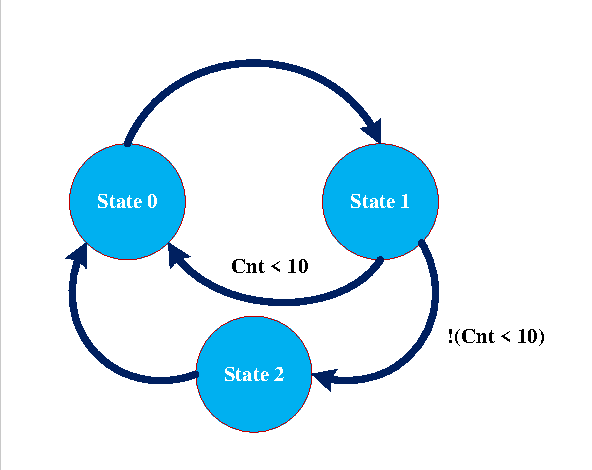
\includegraphics[width=0.4\textwidth]{C:\\Users\\USER\\Documents\\edit_project\\Sobel_Filter\\visio3.pdf}
  \caption{Figure 3}
  \label{fig:visio-diagram}
\end{figure}


% Insert the image in the same section
% \begin{figure}[htbp]
%   \centering
%   \includegraphics[width=0.4\textwidth]{Master_Slave_Diagram.pdf}
%   \caption{Figure 1}
%   \label{fig:visio-diagram}
% \end{figure}

% \begin{description}
% \item[First] This is the first item
% \item[Last] This is the last item
% \end{description}

% \lipsum[9] % Dummy text

\section*{\small{Conclusion}}

% \lipsum[8] % Dummy text

The Sobel Filter implemented in VHDL and synthesized on an FPGA demonstrates the effectiveness of 
hardware-based edge detection. By leveraging hardware acceleration, this project achieves fast, 
real-time processing of images, making it ideal for applications that require quick and accurate edge 
detection, such as object recognition or automated vision systems.

%----------------------------------------------------------------------------------------
%	REFERENCE LIST
%----------------------------------------------------------------------------------------

\begin{thebibliography}{99} % Bibliography - this is intentionally simple in this template

  \bibitem[Alipour Fraydani, 2024]{AlipourFraydani:2024}
  Alipour Fraydani, A. (2024).
  \newblock Homework on Methodology and automatic design algorithms of digital systems, University of Tehran.
  \newblock {\em Unpublished Manuscript}, Department of Electrical Engineering, University of Tehran.
  
\end{thebibliography}

%----------------------------------------------------------------------------------------

\end{document}